\documentclass{article}
\usepackage{amsmath}
\usepackage{graphicx}
\usepackage[margin=1in]{geometry}
\usepackage{enumitem}
\usepackage{xcolor}

\begin{document}
\begin{figure}[h!]
    \begin{minipage}{0.45\textwidth}  % Set the width of the image
        
\includegraphics[width=\textwidth]{ki.png}  % Replace 'image.png' with your image file name
    \end{minipage} \hfill
    \begin{minipage}{0.45\textwidth}  % Set the width of the text block
        \textbf{Name : K.VINOD KUMAR REDDY} \\
    \textbf{Batch : cometfwc0025} \\
  \textbf{Date : 15 MAY 2025}
    \end{minipage}
\end{figure}
\noindent\textbf{Q.38} \quad Refer to the NAND and NOR latches shown in the figure. The inputs ($P_1, P_2$) for both the latches are first made (0,1) and then, after a few seconds, made (1,1). The corresponding stable outputs ($Q_1, Q_2$) are:

\vspace{1em}

\begin{center}
    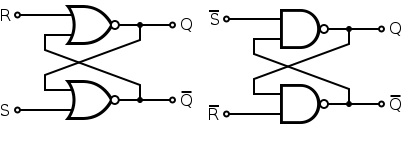
\includegraphics[width=0.8\textwidth]{sr.png} % Ensure sr.png is in the working directory
\end{center}

\vspace{1em}

\begin{enumerate}[label=(\Alph*)]
    \item \begin{tabbing}
        NAND: first (0,1) then (0,1) \quad \= NOR: first (1,0) then (0,0)
    \end{tabbing}
    
    \item \begin{tabbing}
        NAND: first (1,0) then (1,0) \quad \= NOR: first (1,0) then (1,0)
    \end{tabbing}
    
    \item \begin{tabbing}
        NAND: first (1,0) then (1,0) \quad \= NOR: first (1,0) then (0,0)
    \end{tabbing}
    
    \item \begin{tabbing}
        NAND: first (1,0) then (1,1) \quad \= NOR: first (0,1) then (0,1)
    \end{tabbing}
\end{enumerate}

\vspace{1em}

\noindent\textbf{Solution:}

\textbf{NAND Latch (Active-Low SR Latch)}\\
Inputs: $P_1 = S'$, $P_2 = R'$\\
Output: $Q_1$, $Q_2$ (complementary)

\textbf{Truth Table:}
\begin{center}
\begin{tabular}{|c|c|c|c|l|}
\hline
$S'$ & $R'$ & $Q_1$ & $Q_2$ & Description \\
\hline
1 & 1 & No change & No change & Hold state \\
0 & 1 & 1 & 0 & Set \\
1 & 0 & 0 & 1 & Reset \\
0 & 0 & 1 & 1 & Invalid \\
\hline
\end{tabular}
\end{center}

\textbf{Step 1:} Input $(0, 1)$ (Set condition): $Q_1 = 1$, $Q_2 = 0$\\
\textbf{Step 2:} Input $(1, 1)$ (Hold): Output remains $Q_1 = 1$, $Q_2 = 0$

\vspace{0.5em}
\noindent\textbf{Final NAND output:} $(1, 0)$

\vspace{1em}
\textbf{NOR Latch (Active-High SR Latch)}\\
Inputs: $P_1 = S$, $P_2 = R$\\
Output: $Q_1$, $Q_2$ (complementary)

\textbf{Truth Table:}
\begin{center}
\begin{tabular}{|c|c|c|c|l|}
\hline
$S$ & $R$ & $Q_1$ & $Q_2$ & Description \\
\hline
0 & 0 & No change & No change & Hold state \\
1 & 0 & 1 & 0 & Set \\
0 & 1 & 0 & 1 & Reset \\
1 & 1 & 0 & 0 & Invalid \\
\hline
\end{tabular}
\end{center}

\textbf{Step 1:} Input $(0, 1)$ (Reset): $Q_1 = 0$, $Q_2 = 1$\\
\textbf{Step 2:} Input $(1, 1)$ (Invalid): Output becomes $Q_1 = 0$, $Q_2 = 0$

\vspace{0.5em}
\noindent\textbf{Final NOR output:} $(0, 0)$

\vspace{1em}
\noindent\textbf{Answer:} \fcolorbox{black}{yellow!30}{\textbf{(C) NAND: first (1,0) then (1,0); NOR: first (1,0) then (0,0)}}

\end{document}

